\documentclass[11pt]{article}

\usepackage[a4paper,margin=2.3cm]{geometry}
\usepackage[T1]{fontenc}
\usepackage[utf8]{inputenc}
\usepackage{lmodern}
\usepackage{microtype}
\usepackage{amsmath,amssymb}
\usepackage{graphicx}
\usepackage{array}
\usepackage{xcolor}
\usepackage{enumitem}
\setlist{itemsep=2pt,topsep=4pt}
\usepackage{lineno}
\usepackage{listings}
\lstset{basicstyle=\ttfamily\small, columns=fullflexible, keepspaces=true,
  frame=single, rulecolor=\color{black!25}, backgroundcolor=\color{black!3},
  xleftmargin=1.5em, xrightmargin=1.5em, aboveskip=6pt, belowskip=6pt}
\lstdefinestyle{cfg}{basicstyle=\ttfamily\footnotesize}
\usepackage{authblk}
\usepackage[numbers,sort&compress]{natbib}
\usepackage{xr-hyper}
\externaldocument[M-]{../main/main}
\usepackage[colorlinks=true,linkcolor=teal,citecolor=teal,urlcolor=teal]{hyperref}

\title{Supplementary Material for\\ \texttt{Phyloom}: a flexible and extensible framework for simulating phylogenetic trees and networks}
\author[1,2]{Gabriele Marino}
\author[1,2]{Daniele Silvestro}
\author[1,2]{Tanja Stadler}
\affil[1]{Department of Biosystems Science and Engineering, ETH Zurich, Basel, Switzerland}
\affil[2]{SIB Swiss Institute of Bioinformatics, Basel, Switzerland}
\date{}

\renewcommand{\thesection}{S\arabic{section}}
\renewcommand{\thesubsection}{S\arabic{section}.\arabic{subsection}}
\renewcommand{\thefigure}{S\arabic{figure}}
\renewcommand{\thetable}{S\arabic{table}}
\renewcommand{\theequation}{S\arabic{equation}}

\begin{document}
\maketitle
{\small\tableofcontents}
\clearpage
\linenumbers

\section{Birth-death-sampling-hybridization models}
\label{sec:bdsh-models}

The birth-death-sampling-hybridization (\texttt{bdsh}) model simulates a
population of lineages forward in time, from a single ancestor in a given
initial state. Every lineage carries a discrete state label, such as a stage of
infection, a host type, a location, or a trait. Four event rules act on a single
lineage drawn at random, and can be restricted to lineages in a given state:
\texttt{birth} replaces a lineage by two descendants, each keeping the parent's
state or taking a new one; \texttt{death} ends a lineage without observing it;
\texttt{sampling} records a lineage as an observed tip, and either ends it
(sampling with removal) or lets it continue (sampling without removal); and
\texttt{migration} moves a lineage to another state. The three hybridization
rules, \texttt{ldh}, \texttt{lnh}, and \texttt{lgh}, act on a pair of lineages
drawn at random, at a rate per eligible pair, and join the two parents into a
hybrid lineage, differing in whether neither, one, or both parents persist.
Scheduled actions change the population at fixed times instead, for instance
through \texttt{rho\_sample}, which samples each current lineage with a fixed
probability, as in sampling at the present. The resulting history is a tree, or
a network once hybridizations occur.

\subsection{BD: constant rates with a sampling intervention}
\label{ex:bd}

\begin{figure}[ht]
  \centering
  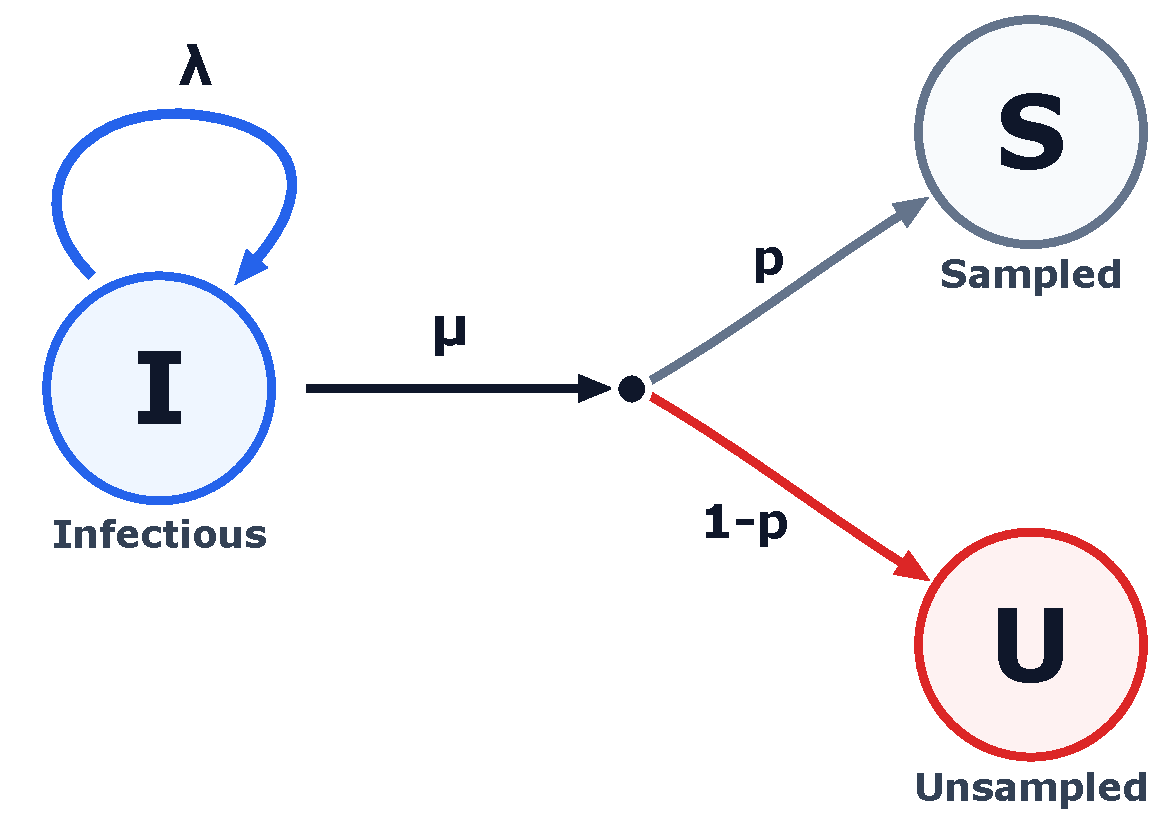
\includegraphics[width=0.6\linewidth]{figures/model-bd.pdf}
  \caption{Birth-Death model.}
  \label{fig:model-bd}
\end{figure}

The constant-rate birth-death model with sampling through
time~\citep{stadler2010sampling}, the simplest phylodynamic model of an
epidemic. Infectious lineages (state \texttt{I}) transmit, i.e.\ branch, at rate
$\lambda$ and are removed (by recovery, death, or isolation) at rate $\mu$; each
removal is sampled with probability $p$. Rather than drawing $\lambda$ directly,
the context draws the basic reproduction number $R_0 = \lambda/\mu$, the
expected number of secondary infections caused by one infected
individual~\citep{stadler2012estimating}, and the mean infectious period
$1/\mu$, and derives $\lambda = R_0\mu$. Removal at total rate $\mu$ is written
as two competing events, unsampled death at rate $\mu(1-p)$ and sampling at rate
$\mu p$. Sampling effort rises at a random intervention time, as when testing is
scaled up during an outbreak: $p$ goes from \texttt{p\_before} to
\texttt{p\_after}, at least twice as large, and both removal rates are
\texttt{skyline} hazards~\citep{stadler2013bdsky} that switch at
\texttt{intervention\_time} and always sum to $\mu$, so the intervention changes
which removals are observed, not the epidemic dynamics. Each trial stops when
\texttt{n\_leaves} tips have been sampled, and is kept only if the epidemic is
still ongoing and at least one tip was sampled before the intervention, so that
the tree informs \texttt{p\_before}. Each sample stores the full history
(\texttt{history.nwk}) and the sampled tree (\texttt{sampled.nwk});
\texttt{metadata.csv} also records the number of tips sampled before the
intervention.

\begin{lstlisting}[style=cfg]
output_dir: outputs/BD-yaml
n_samples: {train: 100, val: 10, test: 10}
n_jobs: -1
seed: 42

context:
  R_0: {type: lognormal, mean: 1.0, sigma: 0.2}
  mu: {type: uniform, low: 0.25, high: 0.6}
  p_before: {type: uniform, low: 0.05, high: 0.15}
  p_after: {type: uniform, low: 2 * p_before, high: 0.5}
  la: R_0 * mu
  psi: mu * np.array([p_before, p_after])
  death_rate: mu - psi
  intervention_time: {type: uniform, low: 4, high: 6}
  n_leaves: {type: integers, low: 20, high: 41}

model:
  spec: bdsh
  init_state: I
  events:
    - rule: {spec: birth}
      hazard: {spec: constant, rate: la}
    - rule: {spec: death}
      hazard: {spec: skyline, rates: death_rate, break_times: [intervention_time]}
    - rule: {spec: sampling, removal: true}
      hazard: {spec: skyline, rates: psi, break_times: [intervention_time]}

stop_criterion: model.count_sampled_lineages() == n_leaves

acceptance_criterion: (
    model.count_current_lineages() > 0
    and any(
      l
      for l in model.get_sampled_lineages()
      if model.time_of(l) < intervention_time
    )
  )

logs:
  n_sampled_before_intervention: sum(
      1
      for l in model.get_sampled_lineages()
      if model.time_of(l) < intervention_time
    )

output_hooks:
  - model.history().dump(output_dir / "history.nwk")
  - model.history(model.get_sampled_lineages()).dump(output_dir / "sampled.nwk")
\end{lstlisting}

\subsection{BDEI: an exposed, non-infectious stage}
\label{ex:bdei}

\begin{figure}[ht]
  \centering
  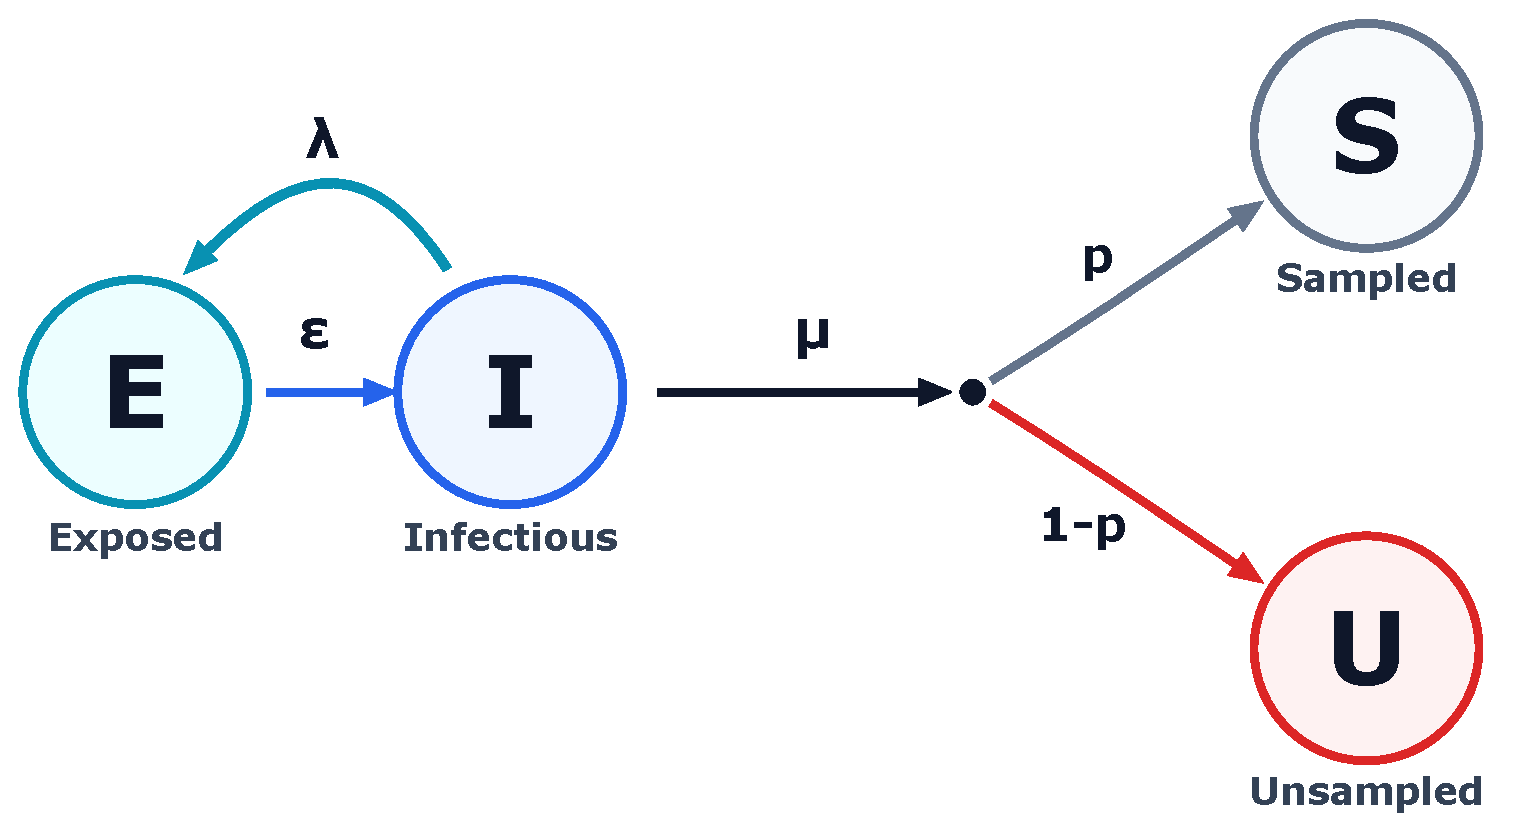
\includegraphics[width=0.6\linewidth]{figures/model-bdei.pdf}
  \caption{Birth-Death Exposed-Infectious model.}
  \label{fig:model-bdei}
\end{figure}

The birth-death exposed-infectious (BDEI) model~\citep{stadler2014ebola} adds an
incubation period to BD, as for pathogens such as Ebola or SARS-CoV-2, where
infected individuals are not infectious straight away. Newly infected lineages
start exposed (state \texttt{E}): they neither transmit nor are removed, and
become infectious (state \texttt{I}) at rate $\varepsilon$. Infectious lineages
transmit at rate $\lambda$, each transmission creating a new \texttt{E} lineage
beside the parent, and are removed at rate $\mu$, each removal sampled with
probability $p$. The \texttt{child\_states} of the \texttt{birth} rule and the
\texttt{migration} rule from \texttt{E} to \texttt{I} are the whole of the
difference from BD. This makes BDEI a multi-type birth-death model, in which
every rate may depend on the state of the
lineage~\citep{stadler2013heterogeneous, kuhnert2016bdmm}.

The context draws the rates through interpretable quantities: $R_0$, the total
duration of infection $T = 1/\varepsilon + 1/\mu$, and the fraction $f$ of it
spent incubating, so that the incubation period is $T_E = fT$, the infectious
period is $T_I = (1-f)T$, and $\lambda = R_0/T_I$. The epidemic starts from an
exposed individual with probability 0.8. Each trial stops when
\texttt{n\_leaves} tips have been sampled, and is kept only if the epidemic is
still ongoing. Each sample stores the sampled tree (\texttt{sampled.nwk});
\texttt{metadata.csv} also records how many lineages are still incubating or
infectious when the trial stops, i.e.\ the unobserved epidemic behind the tree.

\begin{lstlisting}[style=cfg]
output_dir: outputs/BDEI-yaml
n_samples: {train: 100, val: 10, test: 10}
n_jobs: -1
seed: 42

context:
  R_0: {type: lognormal, mean: 1.0, sigma: 0.2}
  T: {type: lognormal, mean: 1.0, sigma: 0.3}
  f: {type: uniform, low: 0.05, high: 0.75}
  T_I: (1 - f) * T
  T_E: f * T
  epsilon: 1 / T_E
  mu: 1 / T_I
  p: {type: uniform, low: 0.05, high: 0.75}
  la: R_0 * mu
  psi: mu * p
  death_rate: mu - psi
  init_state: {type: choice, a: "['E', 'I']", p: "[0.8, 0.2]"}
  n_leaves: {type: integers, low: 50, high: 251}

model:
  spec: bdsh
  init_state: "{init_state}"
  events:
    - rule: {spec: birth, parent_state: I, child_states: [I, E]}
      hazard: {spec: constant, rate: la}
    - rule: {spec: migration, source_state: E, target_state: I}
      hazard: {spec: constant, rate: epsilon}
    - rule: {spec: death, state: I}
      hazard: {spec: constant, rate: death_rate}
    - rule: {spec: sampling, state: I, removal: true}
      hazard: {spec: constant, rate: psi}

stop_criterion: model.count_sampled_lineages() == n_leaves

acceptance_criterion: model.count_current_lineages() > 0

logs:
  still_incubating: model.count_current_lineages("E")
  still_infectious: model.count_current_lineages("I")

output_hooks:
  - model.history(model.get_sampled_lineages()).dump(output_dir / "sampled.nwk")
\end{lstlisting}

\subsection{BDSS: superspreading lineages}
\label{ex:bdss}

\begin{figure}[ht]
  \centering
  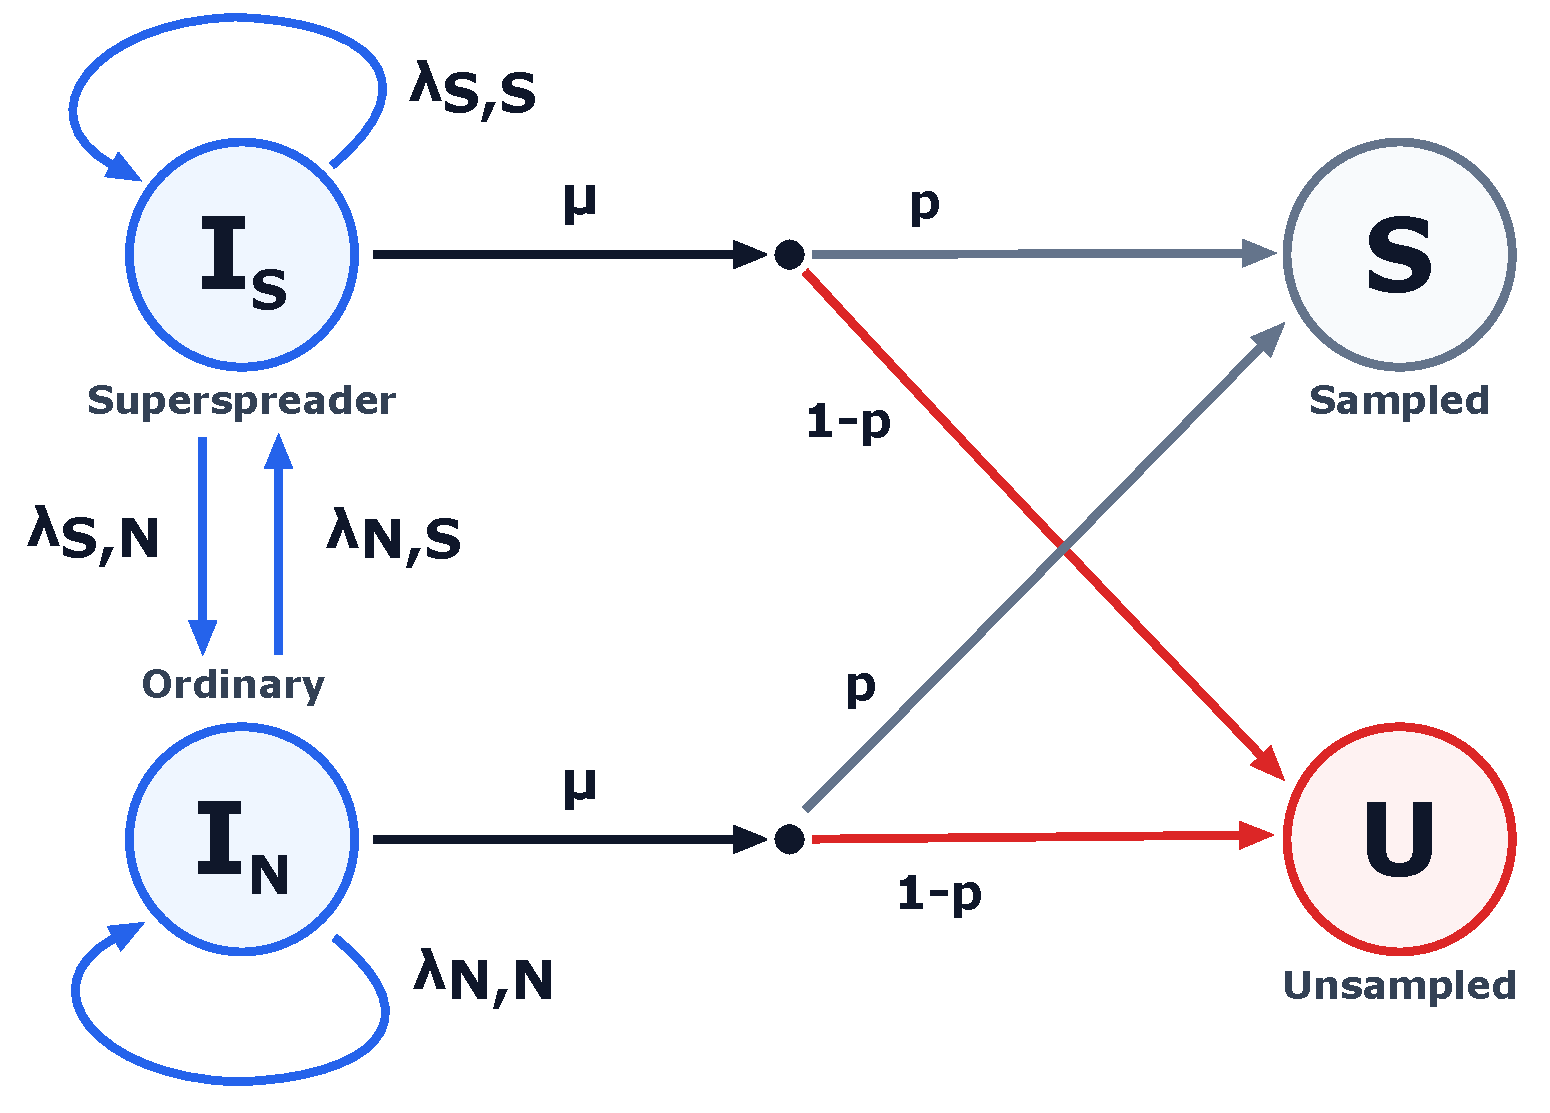
\includegraphics[width=0.6\linewidth]{figures/model-bdss.pdf}
  \caption{Birth-Death super-spreading model.}
  \label{fig:model-bdss}
\end{figure}

The birth-death superspreading (BDSS) model~\citep{stadler2013heterogeneous}
captures heterogeneity in transmission, where a minority of individuals cause a
majority of infections. Infectious lineages are either ordinary (\texttt{I\_N})
or superspreaders (\texttt{I\_S}), and each class can transmit to either class,
giving four birth rates $\lambda_{NN}$, $\lambda_{NS}$, $\lambda_{SN}$, and
$\lambda_{SS}$ (parent class first, offspring class second). Both classes are
removed at the same rate $\mu = 1/T_I$, with $T_I = 2.5$, and sampled with
probability $p = 0.25$.

The context derives those four rates from three interpretable quantities: the
average reproduction number $R_0$; the superspreading fraction $f_{SS}$, the
probability that a new infection is a superspreader, whatever the class of its
infector; and the transmission ratio $r_{SS}$, the factor by which
superspreaders transmit more than ordinary spreaders. Writing $R_{XY} =
  \lambda_{XY}/\mu$, the expressions in the context solve $R_{NS}/(R_{NN}+R_{NS})
  = R_{SS}/(R_{SN}+R_{SS}) = f_{SS}$, $R_{SN}+R_{SS} = r_{SS}(R_{NN}+R_{NS})$, and
$(1-f_{SS})(R_{NN}+R_{NS}) + f_{SS}(R_{SN}+R_{SS}) = R_0$. This kind of
reparameterization keeps priors on quantities one can reason about. The first
lineage is a superspreader with probability $f_{SS}$. Each trial stops when
\texttt{n\_leaves} tips have been sampled, and is kept only if the epidemic is
still ongoing. Each sample stores the sampled tree (\texttt{sampled.nwk});
\texttt{metadata.csv} also records the frequency of superspreaders among the
lineages still infectious at the end of the trial, which approaches $f_{SS}$ in
large outbreaks.

\begin{lstlisting}[style=cfg]
output_dir: outputs/BDSS-yaml
n_samples: {train: 100, val: 10, test: 10}
n_jobs: -1
seed: 42

context:
  R_0: {type: lognormal, mean: 1.0, sigma: 0.2}
  T_I: 2.5
  mu: 1 / T_I
  p: 0.25
  psi: mu * p
  death_rate: mu - psi
  r_SS: {type: uniform, low: 2, high: 10}
  f_SS: {type: uniform, low: 0.1, high: 0.3}
  R_0_NS: R_0 * f_SS / (1 + r_SS * f_SS - f_SS)
  R_0_SN: (R_0 - r_SS * R_0_NS) * r_SS
  R_0_S: r_SS * R_0_NS
  R_0_N: R_0_SN / r_SS
  lambda_NN: R_0_N * mu
  lambda_SS: R_0_S * mu
  lambda_NS: R_0_NS * mu
  lambda_SN: R_0_SN * mu
  init_state: {type: choice, a: "['I_N', 'I_S']", p: "[1 - f_SS, f_SS]"}
  n_leaves: {type: integers, low: 50, high: 251}

model:
  spec: bdsh
  init_state: "{init_state}"
  events:
    - rule: {spec: birth, parent_state: I_N}
      hazard: {spec: constant, rate: lambda_NN}
    - rule: {spec: birth, parent_state: I_S}
      hazard: {spec: constant, rate: lambda_SS}
    - rule: {spec: birth, parent_state: I_N, child_states: [I_N, I_S]}
      hazard: {spec: constant, rate: lambda_NS}
    - rule: {spec: birth, parent_state: I_S, child_states: [I_S, I_N]}
      hazard: {spec: constant, rate: lambda_SN}
    - rule: {spec: death}
      hazard: {spec: constant, rate: death_rate}
    - rule: {spec: sampling, removal: true}
      hazard: {spec: constant, rate: psi}

stop_criterion: model.count_sampled_lineages() == n_leaves

acceptance_criterion: model.count_current_lineages() > 0

logs:
  ss_frequency: model.count_current_lineages("I_S") / model.count_current_lineages()

output_hooks:
  - model.history(model.get_sampled_lineages()).dump(output_dir / "sampled.nwk")
\end{lstlisting}

\subsection{BiSSE: a binary trait driving speciation and extinction}
\label{ex:bisse}

\begin{figure}[ht]
  \centering
  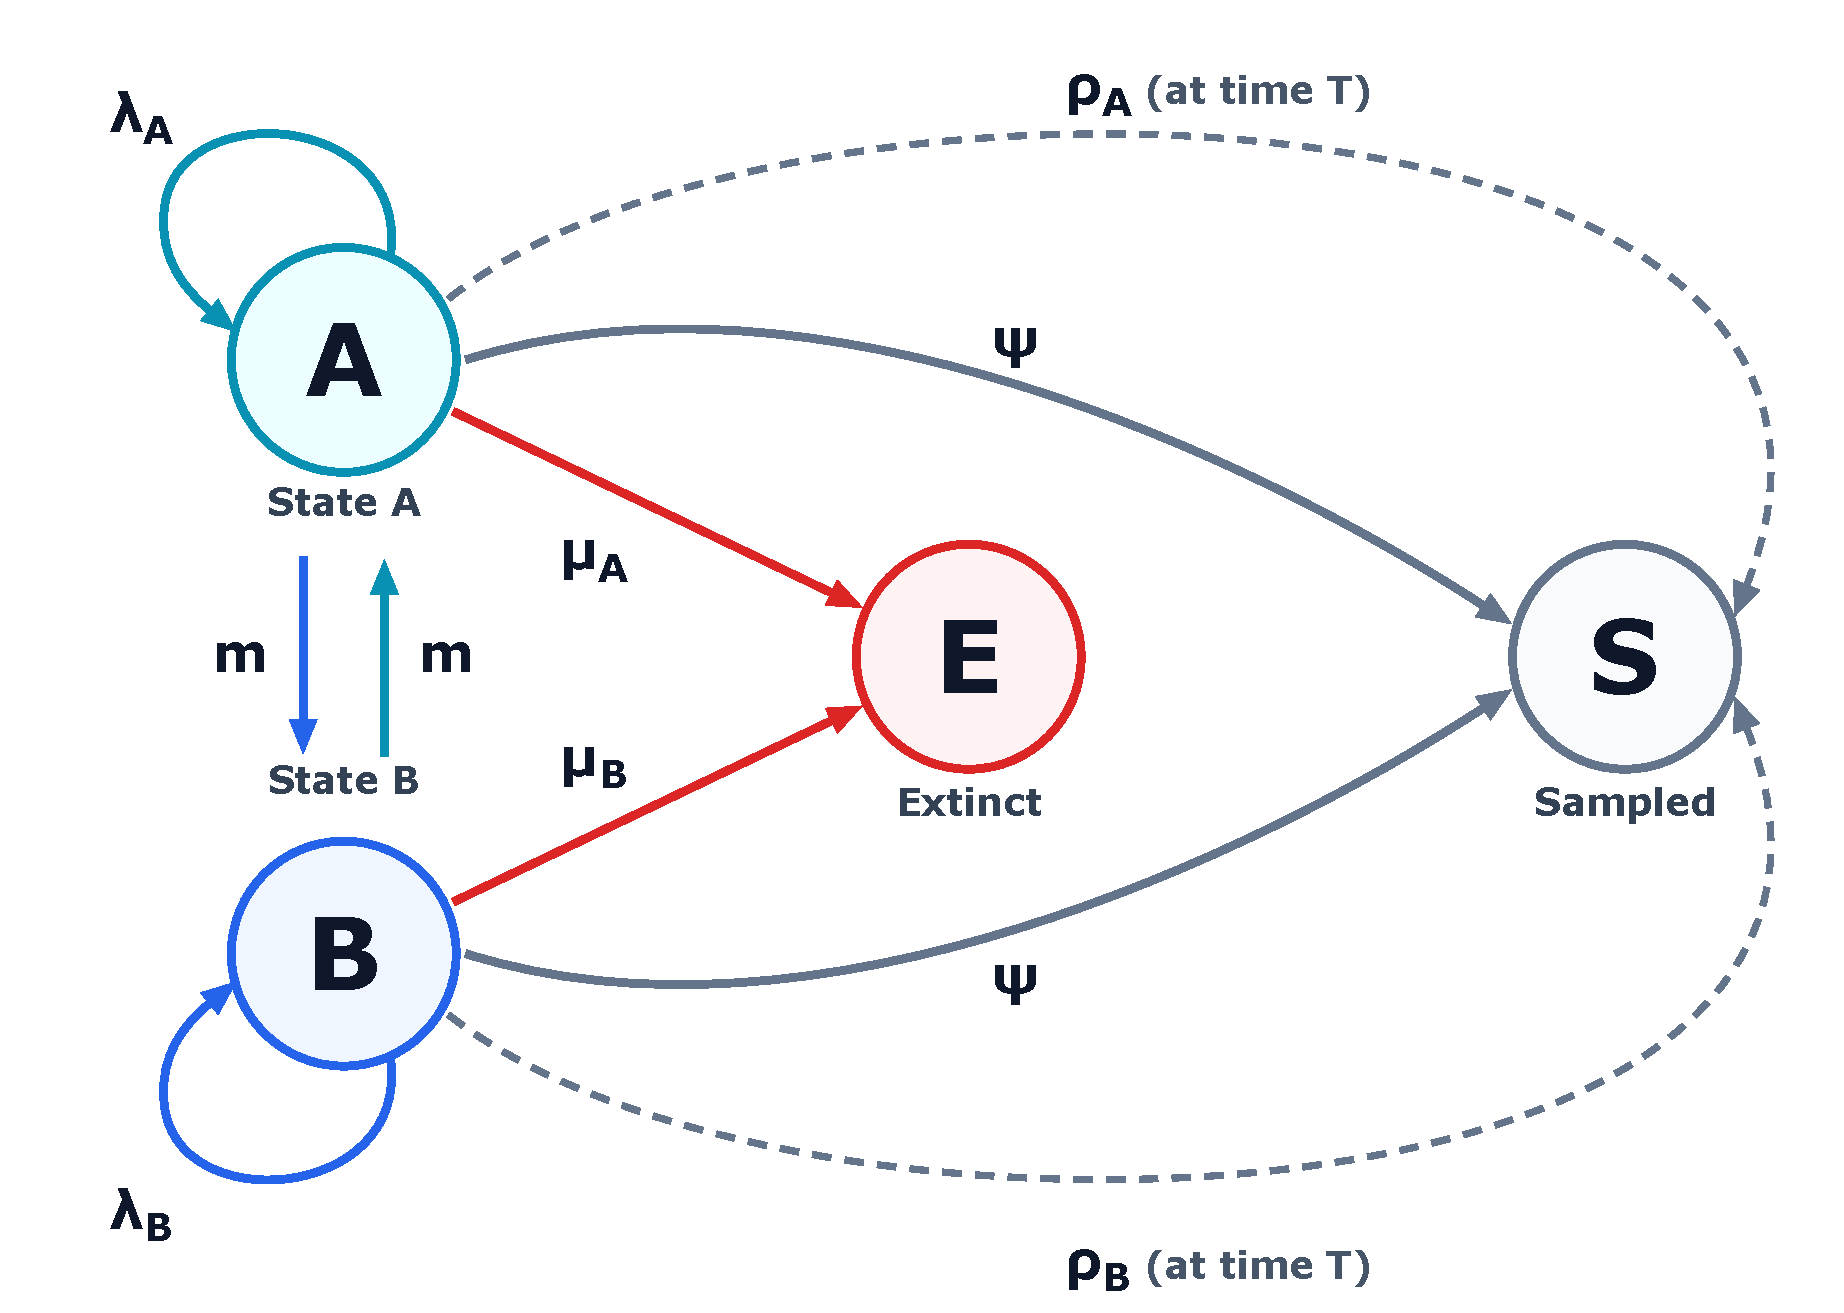
\includegraphics[width=0.6\linewidth]{figures/model-bisse.pdf}
  \caption{BiSSE model.}
  \label{fig:model-bisse}
\end{figure}

The binary-state speciation and extinction (BiSSE)
model~\citep{maddison2007bisse} asks whether a trait, such as a morphological
character or a mode of reproduction, affects the rates at which species
diversify. A binary trait, \texttt{A} or \texttt{B}, sets each lineage's
speciation ($\lambda_A$, $\lambda_B$) and extinction ($\mu_A$, $\mu_B$) rates,
and lineages switch trait at rate $m$ in either direction. The priors make
\texttt{B} speciate up to twice as fast as \texttt{A}, and keep extinction
between a fifth and a half of speciation in both states. The clade is observed
in two ways, as in the fossilized birth-death
process~\citep{heath2014fossilized, gavryushkina2014sampled}: fossil-like
sampling at rate $\psi$ during the simulation, with \texttt{removal: false} so
the lineage survives being sampled and can appear as a sampled ancestor, and a
scheduled action at the present (\texttt{max\_time}) that samples a fraction
$\rho_A$ or $\rho_B$ of the surviving lineages of each state. There is no
\texttt{stop\_criterion}, so every trial runs to \texttt{max\_time} unless the
clade dies out first, and trees vary in size. A trial is kept only if more than
ten tips of each state were sampled. If the parameters of a sample make this too
unlikely, \texttt{max\_rejections} replaces them with a new draw after ten
rejected trials, instead of retrying forever. Each sample stores the sampled
tree (\texttt{sampled.nwk}), with both fossil-like and present-day samples,
whose node labels carry the trait through the tree.

\begin{lstlisting}[style=cfg]
output_dir: outputs/BiSSE-yaml
n_samples: {train: 100, val: 10, test: 10}
n_jobs: -1
seed: 42

context:
  la_A: {type: uniform, low: 0.1, high: 0.3}
  la_B: {type: uniform, low: la_A, high: 2 * la_A}
  mu_A: {type: uniform, low: la_A / 5, high: la_A / 2}
  mu_B: {type: uniform, low: la_B / 5, high: la_B / 2}
  psi: {type: uniform, low: 0.001, high: 0.005}
  m: {type: uniform, low: 0.01, high: 0.05}
  init_state: {type: choice, a: "['A', 'B']", p: "[0.5, 0.5]"}
  max_time: {type: uniform, low: 10, high: 20}
  rho_sample_A: {type: uniform, low: 0.5, high: 0.9}
  rho_sample_B: {type: uniform, low: 0.5, high: 0.9}

model:
  spec: bdsh
  init_state: "{init_state}"
  events:
    - rule: {spec: birth, parent_state: A}
      hazard: {spec: constant, rate: la_A}
    - rule: {spec: birth, parent_state: B}
      hazard: {spec: constant, rate: la_B}
    - rule: {spec: death, state: A}
      hazard: {spec: constant, rate: mu_A}
    - rule: {spec: death, state: B}
      hazard: {spec: constant, rate: mu_B}
    - rule: {spec: migration, source_state: A, target_state: B}
      hazard: {spec: constant, rate: m}
    - rule: {spec: migration, source_state: B, target_state: A}
      hazard: {spec: constant, rate: m}
    - rule: {spec: sampling, removal: false}
      hazard: {spec: constant, rate: psi}
  schedule:
    - times: [max_time]
      action: |
        model.rho_sample(rho_sample_A, "A", removal=False)
        model.rho_sample(rho_sample_B, "B", removal=False)

max_time: max_time

acceptance_criterion: (
    model.count_sampled_lineages("A") > 10
    and model.count_sampled_lineages("B") > 10
  )

max_rejections: 10

output_hooks:
  - model.history(model.get_sampled_lineages()).dump(output_dir / "sampled.nwk")
\end{lstlisting}

\subsection{BDSH: three kinds of hybridization}
\label{sec:bdsh}

This example generates phylogenetic networks under a birth-death process with
hybridization~\citep{zhang2018speciesnetwork, justison2023siphynetwork}.
Hybridization rules act on a pair of lineages and join them into a hybrid
lineage with two parents, so the history is a network rather than a tree.
Lineages branch at rate $\lambda$ and are sampled at rate $\psi$ without being
removed, while pairs of lineages hybridize through three competing
events~\citep{justison2024exploring}: lineage-degenerative hybridization
(\texttt{ldh}), in which the two parents merge into a single hybrid child, so
the number of lineages decreases by one; lineage-neutral hybridization
(\texttt{lnh}), in which one parent persists while the other is absorbed into
the hybrid child, so the number of lineages is unchanged; and lineage-generative
hybridization (\texttt{lgh}), in which both parents persist and the hybrid is a
new lineage, so the number of lineages increases by one. Each kind of hybrid
gets its own state, so the output records which kind of event produced each
reticulation. Hybridization rules act on lineage \emph{pairs} rather than
lineages, so their total rate grows quadratically with the size of the clade.
Each rate is drawn independently for every sample, so the dataset covers
networks dominated by one kind of hybridization as well as mixtures.

Each trial stops when \texttt{n\_leaves} tips have been sampled. A trial is
accepted only if the sampled network really contains a reticulation, that is, if
it has more edges than a tree on the same nodes would (a tree has one edge fewer
than nodes). A hybridization disappears from the sampled network when one of its
parents has no other sampled descendants. Each sample stores the full history
(\texttt{history.nwk}) and the sampled network (\texttt{sampled.nwk}), in
extended Newick; \texttt{metadata.csv} also records the number of tips and
reticulations visible in the sampled network.

\begin{lstlisting}[style=cfg]
output_dir: outputs/BDSH-yaml
n_samples: {train: 10, val: 2, test: 2}
n_jobs: -1
seed: 45

context:
  la: 0.5
  sampling_rate: 0.25
  n_leaves: 50
  ldh_rate: {type: uniform, low: 0.0005, high: 0.003}
  lnh_rate: {type: uniform, low: 0.0005, high: 0.003}
  lgh_rate: {type: uniform, low: 0.0005, high: 0.003}

model:
  spec: bdsh
  init_state: A
  events:
    - rule: {spec: birth}
      hazard: {spec: constant, rate: la}
    - rule: {spec: sampling, removal: false}
      hazard: {spec: constant, rate: sampling_rate}
    - rule: {spec: ldh, hybrid_state: H_LDH}
      hazard: {spec: constant, rate: ldh_rate}
    - rule: {spec: lnh, hybrid_state: H_LNH}
      hazard: {spec: constant, rate: lnh_rate}
    - rule: {spec: lgh, hybrid_state: H_LGH}
      hazard: {spec: constant, rate: lgh_rate}

stop_criterion: model.count_sampled_lineages() == n_leaves

acceptance_criterion: (
    model.history(model.get_sampled_lineages()).n_edges
    > model.history(model.get_sampled_lineages()).n_nodes - 1
  )

logs:
  sampled_tips: model.history(model.get_sampled_lineages()).count_leaves()
  reticulations: (
      model.history(model.get_sampled_lineages()).n_edges
      - model.history(model.get_sampled_lineages()).n_nodes
      + 1
    )

output_hooks:
  - model.history().dump(output_dir / "history.nwk")
  - model.history(model.get_sampled_lineages()).dump(output_dir / "sampled.nwk")
\end{lstlisting}

\subsection{SeasonalBD: a seasonal transmission rate}
\label{sec:seasonal-bd}

Many infections, such as influenza, are transmitted more efficiently in some
seasons than in others. This is a birth-death process whose transmission rate is
a function of time~\citep{kendall1948generalized}, here a seasonal cycle,
\begin{equation*}
  \lambda(t) = \lambda_0\left(1 + a\cos\left(\frac{2\pi(t - t_p)}{P}\right)\right),
\end{equation*}
with mean $\lambda_0 = R_0\mu$, amplitude $a$, period $P$ (one time unit, e.g.\
a year), and peak at $t_p$. Lineages are removed at a constant rate $\mu$ and
each removal is sampled with probability $p$, so only transmission is seasonal.

The built-in hazards are constant, piecewise constant (\texttt{skyline}),
exponential, or a point mass (\texttt{delta}), and none of them covers this
rate. It is therefore given as a plain expression of the simulated time
\texttt{t} through the \texttt{numeric} hazard, which integrates it by
quadrature and inverts the cumulative hazard numerically; firing times are exact
up to the tolerance of the solver, with no discretization of time.
\texttt{initial\_dt} is where the root solver starts bracketing a firing time,
and setting it to a typical waiting time, here $1/\lambda_0$, keeps that search
short. Each trial stops when \texttt{n\_leaves} tips have been sampled, and is
kept only if the epidemic is still ongoing. Each sample stores the full history
(\texttt{history.nwk}) and the sampled tree (\texttt{sampled.nwk});
\texttt{metadata.csv} also records how many tips were sampled while transmission
was above its mean, that is, within a quarter period of a seasonal peak.

\begin{lstlisting}[style=cfg]
output_dir: outputs/SeasonalBD-yaml
n_samples: {train: 100, val: 10, test: 10}
n_jobs: -1
seed: 42

context:
  R_0: {type: lognormal, mean: 1.0, sigma: 0.2}
  mu: {type: uniform, low: 0.25, high: 0.6}
  la_0: R_0 * mu
  amplitude: {type: uniform, low: 0.3, high: 0.9}
  period: 1.0
  peak_time: {type: uniform, low: 0.0, high: 1.0}
  p: {type: uniform, low: 0.1, high: 0.4}
  psi: mu * p
  death_rate: mu - psi
  n_leaves: {type: integers, low: 20, high: 41}

model:
  spec: bdsh
  init_state: I
  events:
    - rule: {spec: birth}
      hazard:
        spec: numeric
        rate_fn: la_0 * (1 + amplitude * np.cos(2 * np.pi * (t - peak_time) / period))
        initial_dt: 1 / la_0
    - rule: {spec: death}
      hazard: {spec: constant, rate: death_rate}
    - rule: {spec: sampling, removal: true}
      hazard: {spec: constant, rate: psi}

stop_criterion: model.count_sampled_lineages() == n_leaves

acceptance_criterion: model.count_current_lineages() > 0

logs:
  n_sampled_in_high_season: sum(
      1
      for l in model.get_sampled_lineages()
      if np.cos(2 * np.pi * (model.time_of(l) - peak_time) / period) > 0
    )

output_hooks:
  - model.history().dump(output_dir / "history.nwk")
  - model.history(model.get_sampled_lineages()).dump(output_dir / "sampled.nwk")
\end{lstlisting}

\subsection{DiversityDependent: diversity dependence and competitive replacement}
\label{sec:diversity-dependent}

\begin{figure}[ht]
  \centering
  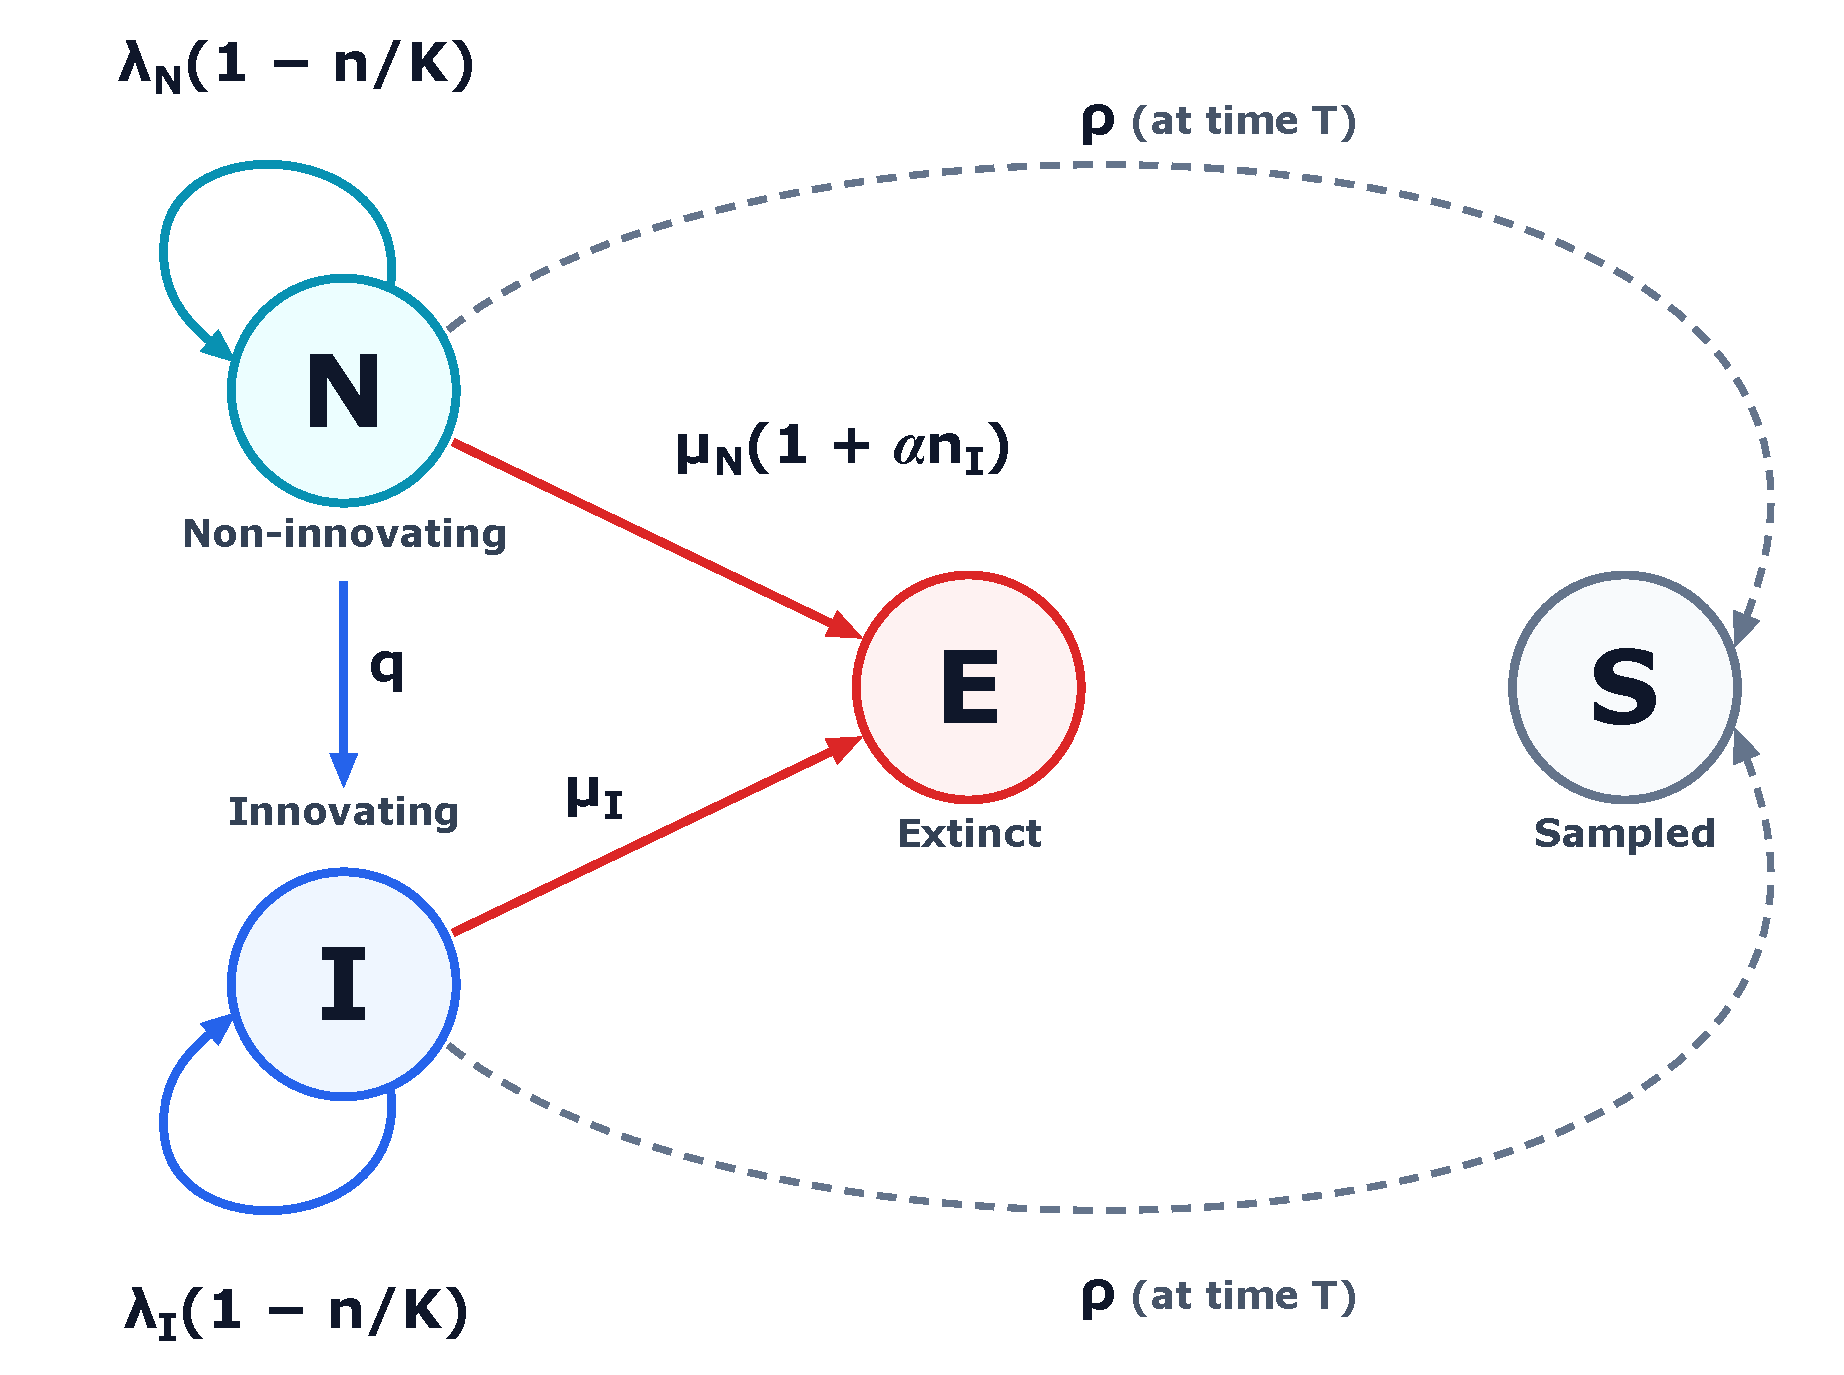
\includegraphics[width=0.6\linewidth]{figures/model-diversity-dependent.pdf}
  \caption{Diversity-dependent model.}
  \label{fig:model-divdep}
\end{figure}

In diversity-dependent models~\citep{rabosky2008density, etienne2012diversity},
speciation slows as a clade fills its ecological niches, so diversity saturates.
This example combines diversity dependence with competitive replacement. A clade
of non-innovating lineages (state \texttt{N}) diversifies until it approaches a
carrying capacity $K$. \texttt{N} lineages acquire a key innovation at rate $q$
and become innovating lineages (state \texttt{I}), which speciate $r_I$ times
faster. With $n$ extant lineages, of which $n_I$ are innovators, the speciation
rate of each state is multiplied by $\max(0, 1 - n/K)$, so speciation stops at
$K$ lineages, and the extinction rate of \texttt{N} lineages by $1 + \alpha
  n_I$, so innovators progressively replace incumbents, with $\alpha$ setting the
strength of competition. Hazards depend only on time, so both multipliers are
\texttt{rate\_multiplier} expressions of the live model, evaluated again before
every step so that the rates follow the state as it changes. There is no
\texttt{stop\_criterion}, so every trial runs to \texttt{max\_time} unless the
clade dies out first. At the present, a scheduled action samples a fraction
$\rho$ of the surviving lineages, and a trial is kept only if at least 20 tips,
5 of them innovators, were sampled. Each sample stores the full history
(\texttt{history.nwk}), which also shows the extinct incumbents, and the sampled
tree (\texttt{sampled.nwk}); \texttt{metadata.csv} also records the number of
extant lineages of each state at the present, which shows how far the
replacement has progressed.

\begin{lstlisting}[style=cfg]
output_dir: outputs/DiversityDependent-yaml
n_samples: {train: 100, val: 10, test: 10}
n_jobs: -1
seed: 42

context:
  K: {type: integers, low: 50, high: 101}
  la_N: {type: uniform, low: 0.2, high: 0.4}
  mu_N: {type: uniform, low: 0.02, high: 0.05}
  r_I: {type: uniform, low: 1.5, high: 3}
  la_I: r_I * la_N
  mu_I: {type: uniform, low: 0.02, high: 0.05}
  q: {type: uniform, low: 0.002, high: 0.01}
  alpha: {type: uniform, low: 0.02, high: 0.1}
  max_time: {type: uniform, low: 40, high: 60}
  rho: {type: uniform, low: 0.5, high: 1.0}

model:
  spec: bdsh
  init_state: N
  events:
    - rule: {spec: birth, parent_state: N}
      hazard: {spec: constant, rate: la_N}
      rate_multiplier: max(0.0, 1 - model.count_current_lineages() / K)
    - rule: {spec: birth, parent_state: I}
      hazard: {spec: constant, rate: la_I}
      rate_multiplier: max(0.0, 1 - model.count_current_lineages() / K)
    - rule: {spec: death, state: N}
      hazard: {spec: constant, rate: mu_N}
      rate_multiplier: 1 + alpha * model.count_current_lineages("I")
    - rule: {spec: death, state: I}
      hazard: {spec: constant, rate: mu_I}
    - rule: {spec: migration, source_state: N, target_state: I}
      hazard: {spec: constant, rate: q}
  schedule:
    - times: [max_time]
      action: |
        model.rho_sample(rho, "N", removal=False)
        model.rho_sample(rho, "I", removal=False)

max_time: max_time

acceptance_criterion: (
    model.count_sampled_lineages() >= 20
    and model.count_sampled_lineages("I") >= 5
  )

logs:
  extant_N: model.count_current_lineages("N")
  extant_I: model.count_current_lineages("I")

output_hooks:
  - model.history().dump(output_dir / "history.nwk")
  - model.history(model.get_sampled_lineages()).dump(output_dir / "sampled.nwk")
\end{lstlisting}

\subsection{BDAliSim: alignments along birth-death trees}
\label{sec:bd-alisim}

This example requires IQ-TREE 3~\citep{wong2026iqtree3}, which provides
AliSim~\citep{lytrong2022alisim}, installed with its \texttt{iqtree3} command on
your \texttt{PATH}. It simulates sampled trees under the constant-rate
birth-death model with sampling through time~\citep{stadler2010sampling}, with
the context drawing $R_0$, the removal rate $\mu$, and the sampling probability
$p$. Each trial stops when \texttt{n\_leaves} tips have been sampled, and is
kept only if the epidemic is still ongoing. A post command, run last for each
sample, then passes the sampled tree to AliSim, which simulates a DNA alignment
along it under the Jukes-Cantor model~\citep{jukes1969evolution}. Branch
lengths, in units of time, are converted into substitutions per site by
\texttt{-{}-branch-scale}, with a strict clock rate drawn for every sample, and
the length of the alignment is drawn uniformly between 500 and 1000 sites. Each
sample stores the sampled tree (\texttt{sampled.nwk}), the simulated alignment
in FASTA format (\texttt{alignment.fa}), and the AliSim log
(\texttt{sampled.nwk.log}).

\begin{lstlisting}[style=cfg]
output_dir: outputs/BDAliSim-yaml
n_samples: {train: 100, val: 10, test: 10}
n_jobs: -1
seed: 42

context:
  R_0: {type: uniform, low: 1.5, high: 4.0}
  mu: {type: uniform, low: 0.25, high: 0.6}
  p: {type: uniform, low: 0.1, high: 0.5}
  la: R_0 * mu
  death_rate: mu * (1 - p)
  psi: mu * p
  n_leaves: {type: integers, low: 20, high: 41}
  clock_rate: {type: uniform, low: 0.001, high: 0.01}
  seq_length: {type: integers, low: 500, high: 1001}
  alisim_seed: {type: integers, low: 1, high: 2**31}

model:
  spec: bdsh
  init_state: I
  events:
    - rule: {spec: birth}
      hazard: {spec: constant, rate: la}
    - rule: {spec: death}
      hazard: {spec: constant, rate: death_rate}
    - rule: {spec: sampling, removal: true}
      hazard: {spec: constant, rate: psi}

stop_criterion: model.count_sampled_lineages() == n_leaves

acceptance_criterion: model.count_current_lineages() > 0

output_hooks:
  - model.history(model.get_sampled_lineages()).dump(output_dir / "sampled.nwk")

post_commands:
  - iqtree3 --alisim {output_dir}/alignment -t {output_dir}/sampled.nwk
    -m JC --length {seq_length} --branch-scale {clock_rate}
    --seed {alisim_seed} -af fasta
\end{lstlisting}

% -----------------------------------------------------------------------------
\section{The coalescent}
\label{sec:coalescent-models}

Coalescent models describe the genealogy of a sample backward in time, from the
sampled lineages to their most recent common
ancestor~\citep{kingman1982coalescent}, without simulating the rest of the
population. The \texttt{coalescent} model starts from an initial set of sampled
lineages per state, such as demes, and has two event rules, both of which can be
restricted to lineages in given states: \texttt{coalesce} merges a pair of
lineages into their common ancestor, at a rate per eligible pair that is
inversely proportional to the effective population size, so that changes in
population size are expressed through a time-varying rate; and \texttt{retrace}
moves a single lineage to another state, as a migration traced backward in time.
Samples taken further in the past are added by scheduled actions that call
\texttt{spawn}, which adds a new sampled lineage at the scheduled time, giving
serially sampled tips.

\subsection{Coalescent: a single population of constant size}
\label{ex:coalescent}

The Kingman coalescent~\citep{kingman1982coalescent} describes the genealogy of
a sample of lineages drawn from a large, well-mixed population of constant
effective size $N_e$, and is simulated backward in time, from the samples to
their most recent common ancestor. Between 8 and 12 lineages are sampled at the
present. Each pair of lineages merges at rate $1/(2N_e)$, with time measured in
generations, and counting every pair supplies the $\binom{n}{2}$ factor of the
Kingman coalescent, so the total coalescence rate falls from
$\binom{n}{2}/(2N_e)$ as lineages merge. The simulation stops when a single
lineage, the root, is left. Each sample stores the genealogy
(\texttt{genealogy.nwk}).

\begin{lstlisting}[style=cfg]
output_dir: outputs/Coalescent-yaml
n_samples: {train: 10, val: 2, test: 2}
n_jobs: -1
seed: 42

context:
  n_tips: {type: integers, low: 8, high: 13}
  effective_population_size: 100
  coalescence_rate: 1 / (2 * effective_population_size)

model:
  spec: coalescent
  init_population: {A: n_tips}
  events:
    - rule: {spec: coalesce, current_states: [A, A], ancestral_state: A}
      hazard: {spec: constant, rate: coalescence_rate}

stop_criterion: model.count_current_lineages() == 1

output_hooks:
  - model.history().dump(output_dir / "genealogy.nwk")
\end{lstlisting}

\subsection{SerialCoalescent: serially sampled tips}
\label{ex:serialcoal}

In many datasets, samples are not all collected at the same time: ancient DNA,
or pathogens sequenced throughout an epidemic, give serially sampled, or
heterochronous, tips~\citep{drummond2002serial}. Backward in time, such a sample
enters the genealogy at its sampling time, and from then on can only coalesce
with lineages that are still being traced. Here, between 4 and 8 lineages are
sampled at the present, and between 4 and 8 further lineages at times drawn
uniformly between the present and $2N_e$ generations in the past, within the
expected depth of the genealogy. Each of them is added at its sampling time by a
scheduled action that calls \texttt{spawn}. The genealogy may coalesce into a
single lineage before all samples are added, so the stop criterion also requires
the oldest sample to have been added; until then, the single remaining lineage
is simply traced further back. Each sample stores the genealogy
(\texttt{genealogy.nwk}), whose tips lie at their sampling times;
\texttt{metadata.csv} also records the time to the most recent common ancestor.

\begin{lstlisting}[style=cfg]
output_dir: outputs/SerialCoalescent-yaml
n_samples: {train: 10, val: 2, test: 2}
n_jobs: -1
seed: 46

context:
  n_present: {type: integers, low: 4, high: 9}
  n_past: {type: integers, low: 4, high: 9}
  effective_population_size: 100
  coalescence_rate: 1 / (2 * effective_population_size)
  sampling_times: {type: uniform, low: 0, high: 2 * effective_population_size, size: n_past}
  oldest_sampling_time: sampling_times.max()

model:
  spec: coalescent
  init_population: {A: n_present}
  events:
    - rule: {spec: coalesce, current_states: [A, A], ancestral_state: A}
      hazard: {spec: constant, rate: coalescence_rate}
  schedule:
    - times: sampling_times
      action: model.spawn("A")

stop_criterion: (
    model.current_time >= oldest_sampling_time
    and model.count_current_lineages() == 1
  )

logs:
  tmrca: model.current_time

output_hooks:
  - model.history().dump(output_dir / "genealogy.nwk")
\end{lstlisting}

\subsection{StructuredCoalescent: two demes connected by migration}
\label{ex:structcoal}

The structured coalescent~\citep{takahata1988coalescent, notohara1990coalescent}
extends the coalescent to a population subdivided into demes, such as geographic
locations or host species, between which individuals migrate. Four lineages are
sampled from each of two demes, \texttt{A} and \texttt{B}, of the same effective
size, connected by symmetric migration. Backward in time, lineages coalesce only
within their deme, at the same pairwise rate as in a single population, and
\texttt{retrace} rules move them between demes at a constant rate, so two
lineages in different demes must come to share a deme before they can merge. As
time runs backward, a \texttt{retrace} from \texttt{A} to \texttt{B} means that
the ancestor belonged to deme \texttt{B}: forward in time, a migration from
\texttt{B} into \texttt{A}. The stop criterion is essential here, since
\texttt{retrace} events would otherwise keep firing on the root forever. Each
sample stores the genealogy (\texttt{genealogy.nwk}), in which each
\texttt{retrace} is kept as a node with one child, and node labels carry the
deme, recording the deme of each ancestral lineage over time.

\begin{lstlisting}[style=cfg]
output_dir: outputs/StructuredCoalescent-yaml
n_samples: {train: 10, val: 2, test: 2}
n_jobs: -1
seed: 43

context:
  effective_population_size: 1
  coalescence_rate: 1 / (2 * effective_population_size)
  migration_rate: 0.5

model:
  spec: coalescent
  init_population: {A: 4, B: 4}
  events:
    - rule: {spec: retrace, current_state: A, ancestral_state: B}
      hazard: {spec: constant, rate: migration_rate}
    - rule: {spec: retrace, current_state: B, ancestral_state: A}
      hazard: {spec: constant, rate: migration_rate}
    - rule: {spec: coalesce, current_states: [A, A], ancestral_state: A}
      hazard: {spec: constant, rate: coalescence_rate}
    - rule: {spec: coalesce, current_states: [B, B], ancestral_state: B}
      hazard: {spec: constant, rate: coalescence_rate}

stop_criterion: model.count_current_lineages() == 1

output_hooks:
  - model.history().dump(output_dir / "genealogy.nwk")
\end{lstlisting}

\subsection{ExponentialGrowthCoalescent: an exponentially growing population}
\label{ex:expcoal}

A coalescent with a time-varying effective population
size~\citep{griffiths1994varying, slatkin1991pairwise}, here for a population,
such as an expanding epidemic, that has grown exponentially at rate $g$ up to
the present size $N_e(0)$. Backward in time, the effective size $N_e(t) =
  N_e(0)\,e^{-gt}$ shrinks and the pairwise coalescence rate $1/(2N_e(t))$ grows
as $e^{gt}$. That is an \texttt{exponential} hazard with a negative
\texttt{decay}. Because coalescence is rare near the present and fast in the
small ancestral population, the genealogies are star-like, with long terminal
branches and ancestors compressed near the root. The simulation stops when a
single lineage, the root, is left. Each sample stores the genealogy
(\texttt{genealogy.nwk}).

\begin{lstlisting}[style=cfg]
output_dir: outputs/ExponentialGrowthCoalescent-yaml
n_samples: {train: 10, val: 2, test: 2}
n_jobs: -1
seed: 44

context:
  n_tips: {type: integers, low: 8, high: 13}
  present_effective_population_size: 1000
  growth_rate: 0.1
  coalescence_rate_at_present: 1 / (2 * present_effective_population_size)
  hazard_decay: -growth_rate

model:
  spec: coalescent
  init_population: {A: n_tips}
  events:
    - rule: {spec: coalesce}
      hazard:
        spec: exponential
        rate: coalescence_rate_at_present
        decay: hazard_decay

stop_criterion: model.count_current_lineages() == 1

output_hooks:
  - model.history().dump(output_dir / "genealogy.nwk")
\end{lstlisting}

% -----------------------------------------------------------------------------
\section{Compartmental epidemics}
\label{sec:epidemic-models}

Compartmental models describe an epidemic in a finite host
population~\citep{kermack1927contribution, hethcote2000mathematics}, so that
transmission slows down as susceptible hosts are depleted. The \texttt{epidemic}
model keeps uninfected compartments, such as susceptible and recovered hosts, as
pools of plain counts, and infected hosts as lineages, so that only the
transmission tree is recorded in full. Its event rules act on lineages, on hosts
in a pool, or on both: \texttt{infection} takes a host from a pool, e.g.\
susceptible, and adds a new lineage beside its infector, at a rate per pair of
an infected lineage and a host in that pool, so that transmission slows as the
pool empties; \texttt{recovery} ends a lineage, optionally sampling it, and
returns the host to a pool, e.g.\ recovered; \texttt{migration} moves a lineage
to another state, e.g.\ from exposed to infectious; and \texttt{flow} moves a
host from one pool to another, e.g.\ when immunity wanes, at a rate per host in
the source pool. The rules that act on lineages can be restricted to lineages in
a given state.

\subsection{SIR: susceptible, infectious, recovered}
\label{ex:sir}

\begin{figure}[ht]
  \centering
  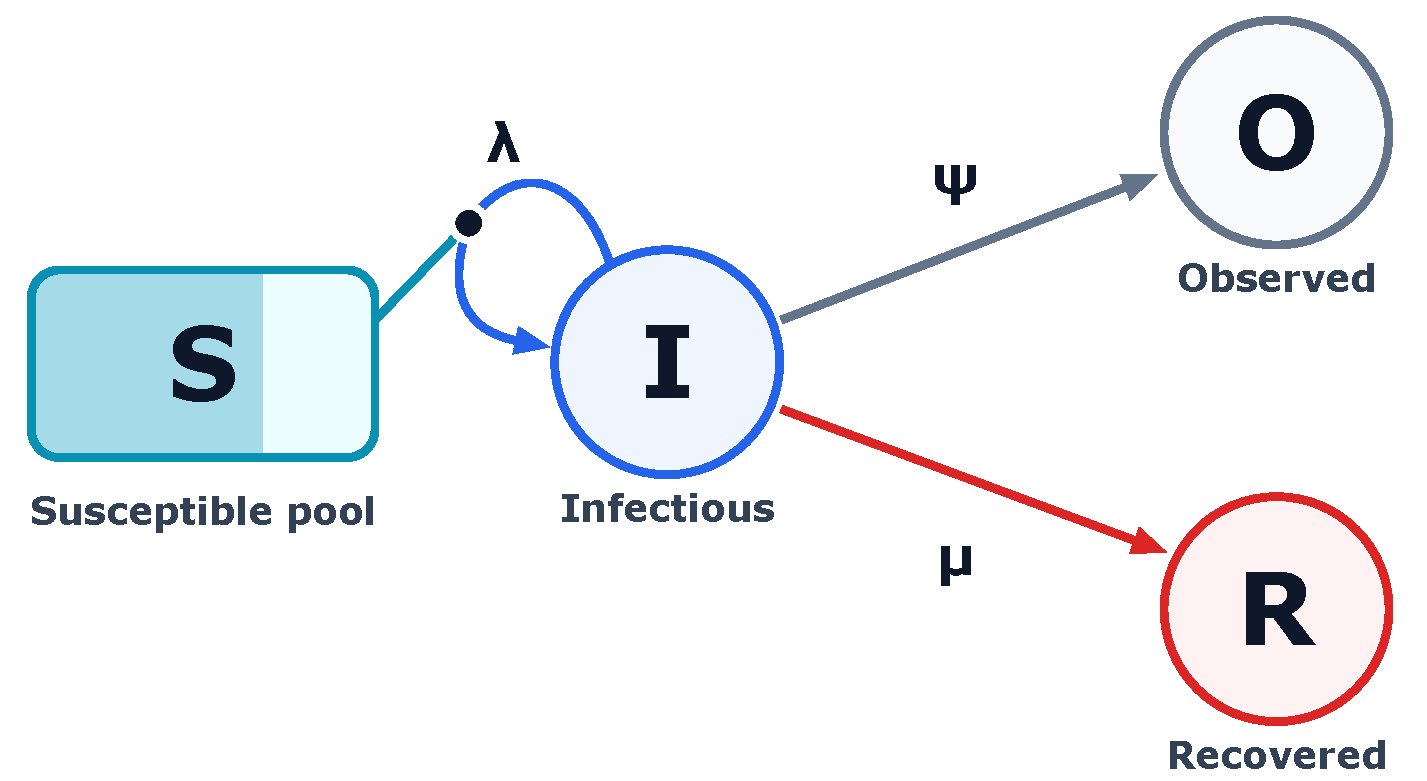
\includegraphics[width=0.6\linewidth]{figures/model-sir.pdf}
  \caption{SIR model.}
  \label{fig:model-sir}
\end{figure}

The susceptible-infectious-recovered (SIR) model~\citep{kermack1927contribution,
  hethcote2000mathematics} describes an epidemic in a closed host population,
which slows down and eventually burns out as susceptible hosts are depleted.
Here it produces a transmission tree, as in phylodynamic analyses of
density-dependent transmission~\citep{leventhal2014density, kuhnert2014bdsir}.
Susceptible (\texttt{S}) and recovered (\texttt{R}) hosts are pools, counted but
not tracked individually; infectious hosts are lineages in state \texttt{I}. An
infection consumes one susceptible host and creates a new \texttt{I} lineage,
and an \texttt{I} lineage recovers into \texttt{R}, either unobserved at rate
$\mu$ or sampled at rate $\psi$, so that a fraction $s$ of recoveries are
sampled. The \texttt{infection} rule counts every pair of an infectious lineage
and a susceptible host, so the per-lineage transmission rate is $\lambda S$ and
decreases as the epidemic depletes $S$. The context sets $\lambda =
  R_0(\mu+\psi)/S_0$, so that $R_0$ is the reproduction number at the start of the
epidemic, in a population of $S_0$ susceptible hosts. The trial stops at the
twentieth sample, so the trees mostly describe the growth phase, and is kept
only if the epidemic is still ongoing. Each sample stores the sampled tree
(\texttt{sampled.nwk}); \texttt{metadata.csv} also records the final sizes of
the susceptible and recovered pools, which show
how far the epidemic has depleted the susceptible pool.

\begin{lstlisting}[style=cfg]
output_dir: outputs/SIR-yaml
n_samples: {train: 100, val: 10, test: 10}
n_jobs: -1
seed: 42

context:
  R_0: {type: uniform, low: 1.5, high: 4}
  exit_rate: {type: uniform, low: 0.05, high: 0.2}
  s: {type: uniform, low: 0.2, high: 0.5}
  mu: exit_rate * (1 - s)
  psi: exit_rate * s
  init_S: {type: integers, low: 200, high: 1001}
  la: R_0 * exit_rate / init_S

model:
  spec: epidemic
  init_state: I
  init_pools: {S: init_S}
  events:
    - rule: {spec: infection, recipient_pool: S}
      hazard: {spec: constant, rate: la}
    - rule: {spec: recovery, destination_pool: R}
      hazard: {spec: constant, rate: mu}
    - rule: {spec: recovery, destination_pool: R, sample: true}
      hazard: {spec: constant, rate: psi}

stop_criterion: model.count_sampled_lineages() == 20

acceptance_criterion: model.count_current_lineages() > 0

logs:
  still_susceptible: model.pools["S"]
  recovered: model.pools["R"]

output_hooks:
  - model.history(model.get_sampled_lineages()).dump(output_dir / "sampled.nwk")
\end{lstlisting}

\subsection{SEIR: an incubation stage}
\label{ex:seir}

\begin{figure}[ht]
  \centering
  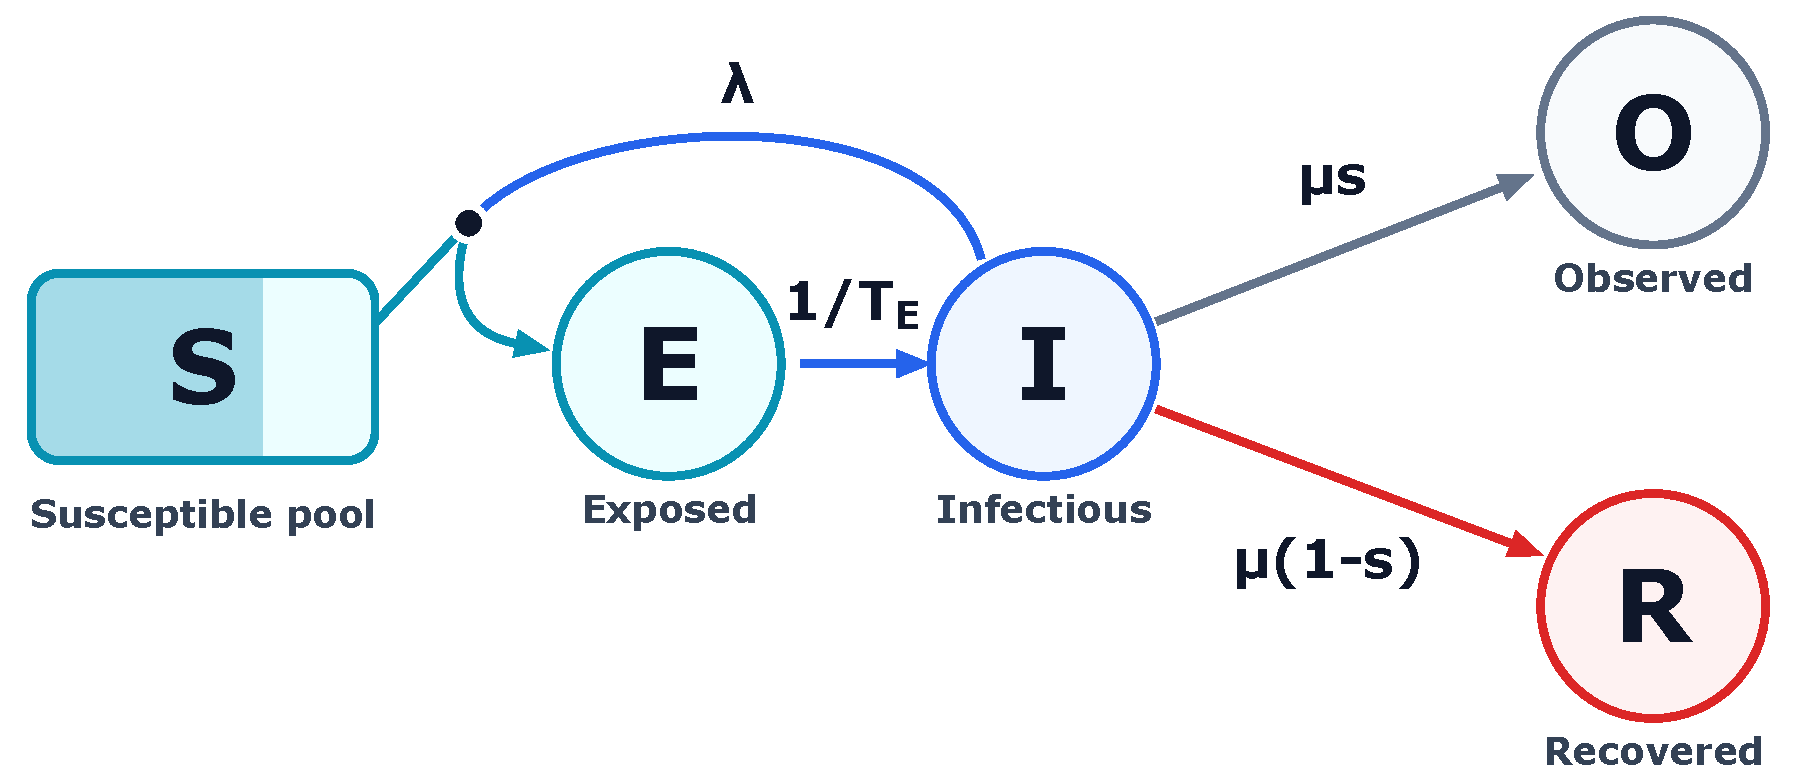
\includegraphics[width=0.6\linewidth]{figures/model-seir.pdf}
  \caption{SEIR model.}
  \label{fig:model-seir}
\end{figure}

SIR with infected hosts split into exposed (\texttt{E}: infected but not yet
infectious) and infectious (\texttt{I}) lineages. Infections create \texttt{E}
lineages, which become infectious after a mean time $T_E$; \texttt{I} lineages
recover at rate $\mu = 1/T_I$, a fraction $s$ of them sampled. As in SIR,
$\lambda = R_0\mu/S_0$ makes $R_0$ the initial reproduction number. The trial
stops at the twentieth sample, and is kept only if the epidemic is still
ongoing. Each sample stores the sampled tree (\texttt{sampled.nwk});
\texttt{metadata.csv} also records the final sizes of the susceptible and
recovered pools and the number of lineages still incubating.

\begin{lstlisting}[style=cfg]
output_dir: outputs/SEIR-yaml
n_samples: {train: 100, val: 10, test: 10}
n_jobs: -1
seed: 42

context:
  R_0: {type: uniform, low: 1.5, high: 4}
  T_E: {type: uniform, low: 1, high: 5}
  T_I: {type: uniform, low: 5, high: 20}
  mu: 1 / T_I
  s: {type: uniform, low: 0.2, high: 0.5}
  init_S: {type: integers, low: 200, high: 1001}
  la: R_0 * mu / init_S

model:
  spec: epidemic
  init_state: I
  init_pools: {S: init_S}
  events:
    - rule: {spec: infection, recipient_pool: S, source_state: I, child_states: [I, E]}
      hazard: {spec: constant, rate: la}
    - rule: {spec: recovery, source_state: I, destination_pool: R}
      hazard: {spec: constant, rate: mu * (1 - s)}
    - rule: {spec: recovery, source_state: I, destination_pool: R, sample: true}
      hazard: {spec: constant, rate: mu * s}
    - rule: {spec: migration, source_state: E, target_state: I}
      hazard: {spec: constant, rate: 1 / T_E}

stop_criterion: model.count_sampled_lineages() == 20

acceptance_criterion: model.count_current_lineages() > 0

logs:
  still_susceptible: model.pools["S"]
  recovered: model.pools["R"]
  still_incubating: model.count_current_lineages("E")

output_hooks:
  - model.history(model.get_sampled_lineages()).dump(output_dir / "sampled.nwk")
\end{lstlisting}

\subsection{SEIRS: waning immunity}
\label{ex:seirs}

\begin{figure}[ht]
  \centering
  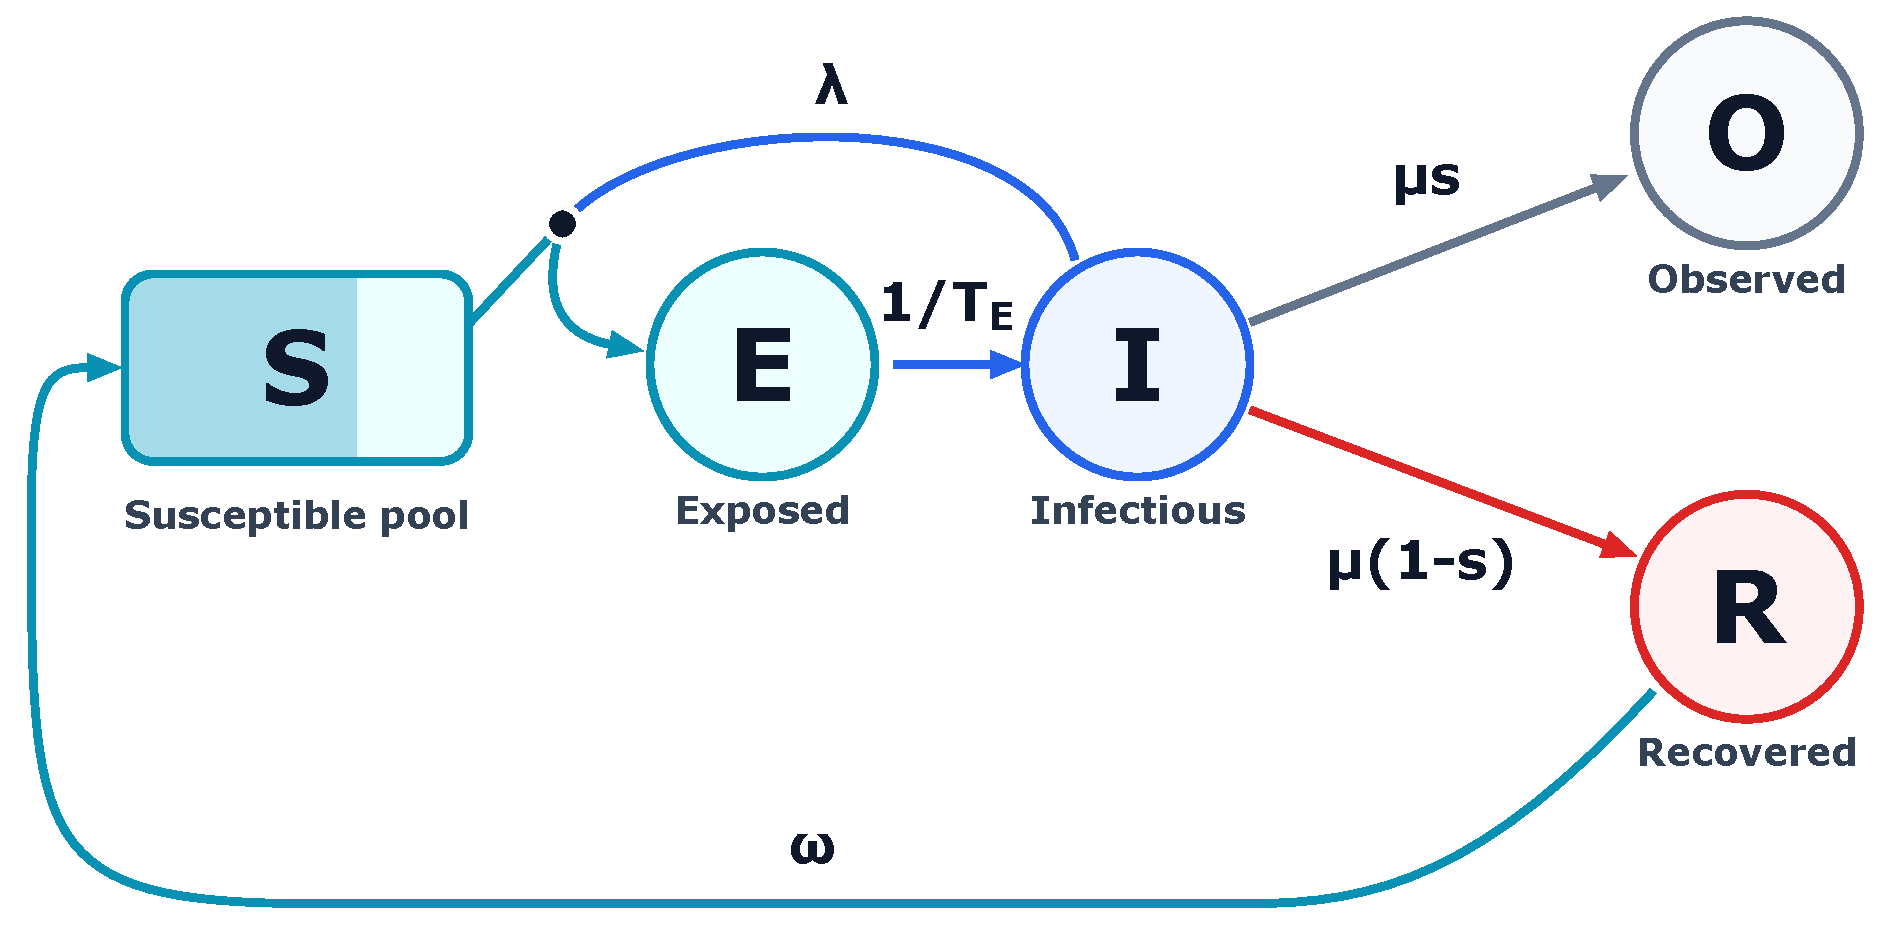
\includegraphics[width=0.6\linewidth]{figures/model-seirs.pdf}
  \caption{SEIRS model.}
  \label{fig:model-seirs}
\end{figure}

SEIR with a \texttt{flow} rule that returns each recovered host to the
susceptible pool at rate $\omega = 1/T_R$, where $T_R$ is the mean duration of
immunity. Waning replenishes \texttt{S}, so the epidemic can persist instead of
burning out. The trial stops at the hundredth sample, and is kept only if the
epidemic is still ongoing. Each sample stores the sampled tree
(\texttt{sampled.nwk}); \texttt{metadata.csv} also records the final sizes of
the susceptible and recovered pools and the number of lineages still incubating.

\begin{lstlisting}[style=cfg]
output_dir: outputs/SEIRS-yaml
n_samples: {train: 100, val: 10, test: 10}
n_jobs: -1
seed: 42

context:
  R_0: {type: uniform, low: 1.5, high: 4}
  T_E: {type: uniform, low: 1, high: 5}
  T_I: {type: uniform, low: 5, high: 20}
  T_R: {type: uniform, low: 3 * T_I, high: 10 * T_I}
  omega: 1 / T_R
  mu: 1 / T_I
  s: {type: uniform, low: 0.2, high: 0.5}
  init_S: {type: integers, low: 100, high: 200}
  la: R_0 * mu / init_S

model:
  spec: epidemic
  init_state: I
  init_pools: {S: init_S}
  events:
    - rule: {spec: infection, recipient_pool: S, source_state: I, child_states: [I, E]}
      hazard: {spec: constant, rate: la}
    - rule: {spec: recovery, source_state: I, destination_pool: R}
      hazard: {spec: constant, rate: mu * (1 - s)}
    - rule: {spec: recovery, source_state: I, destination_pool: R, sample: true}
      hazard: {spec: constant, rate: mu * s}
    - rule: {spec: migration, source_state: E, target_state: I}
      hazard: {spec: constant, rate: 1 / T_E}
    - rule: {spec: flow, source_pool: R, destination_pool: S}
      hazard: {spec: constant, rate: omega}

stop_criterion: model.count_sampled_lineages() == 100

acceptance_criterion: model.count_current_lineages() > 0

logs:
  still_susceptible: model.pools["S"]
  recovered: model.pools["R"]
  still_incubating: model.count_current_lineages("E")

output_hooks:
  - model.history(model.get_sampled_lineages()).dump(output_dir / "sampled.nwk")
\end{lstlisting}

% -----------------------------------------------------------------------------
\section{Plugins}
\label{sec:app-plugins}

A plugin is an installable Python package that extends Phyloom with new
functionality, such as a model or event rules, and registers it so that it can
be used in YAML configurations. Once a plugin is installed, the \texttt{phyloom}
command runs its configurations with all the usual machinery: parameter priors,
stopping and acceptance criteria, parallel sample generation, logs, and output
hooks. A plugin is needed when a process requires something the built-in models
cannot express, such as state that belongs to individuals (identities, contact
histories, or ages), waiting times that belong to a single lineage
(non-exponential lifetimes), or events that trigger other events depending on
the model's history (tracing the contacts of a sampled individual).

\subsection{Age-dependent branching}
\label{sec:age-dependent-branching}

In a binary age-dependent branching process, also known as a Bellman-Harris
process~\citep{harris1963theory}, every individual lives for a random lifetime
drawn from a general distribution. At the end of its life, it either dies or
splits into two new individuals, which start their own lifetimes from age zero.
The classic application is cell proliferation, in which a cell that has just
divided is unlikely to divide again immediately, and whose history can be
recorded as a cell lineage tree by genetic lineage
tracing~\citep{seidel2022tidetree}. This plugin simulates the multi-type version
of the process:

\begin{enumerate}
  \item Every lineage carries a discrete state, such as \texttt{A} or
        \texttt{B}.
  \item When a lineage begins, it draws its lifetime from a distribution that
        depends on its state.
  \item At the end of the lifetime, it dies with a state-dependent probability.
  \item Otherwise, it is replaced by two descendants, whose states follow a
        configurable transition rule, and which start fresh lifetimes.
\end{enumerate}

With non-exponential lifetimes, such as Gamma lifetimes with shape greater than
one, the remaining lifetime of a lineage that has already lived for a while
follows a different distribution than the lifetime of a newborn one. The chance
that a lineage branches in the next instant therefore depends on its
\emph{age}.

\subsubsection*{Example}

Two states, \texttt{A} and \texttt{B}, with Gamma lifetimes (fixed shapes above
one, mean drawn per sample), state-specific death probabilities, and independent
state switches of the two descendants at each split. Trials run up to a maximum
time and are kept if at least a minimum number of lineages is still alive; each
sample stores the full history tree and the number of extant lineages per state.

\begin{lstlisting}[style=cfg]
output_dir: outputs/ADB-multistate
n_samples: {train: 100, val: 10, test: 10}
n_jobs: -1
seed: 42

context:
  mean_lifetime_A: {type: uniform, low: 1.2, high: 1.8}
  mean_lifetime_B: {type: uniform, low: 0.7, high: 1.1}
  shape_A: 3.0
  shape_B: 4.0
  scale_A: mean_lifetime_A / shape_A
  scale_B: mean_lifetime_B / shape_B
  death_prob_A: {type: uniform, low: 0.35, high: 0.50}
  death_prob_B: {type: uniform, low: 0.45, high: 0.60}
  p_A_to_B: {type: uniform, low: 0.10, high: 0.35}
  p_B_to_A: {type: uniform, low: 0.10, high: 0.35}
  init_state: {type: choice, a: "['A', 'B']", p: "[0.5, 0.5]"}

model:
  spec: adb
  init_state: "{init_state}"
  lifetime_func: >-
    model.rng.gammavariate(
      shape_A if state == "A" else shape_B,
      scale_A if state == "A" else scale_B
    )
  death_prob: death_prob_A if state == "A" else death_prob_B
  get_child_states: >-
    model.rng.choices(
      ["A", "B"],
      weights=[1 - p_A_to_B, p_A_to_B] if state == "A" else
              [p_B_to_A, 1 - p_B_to_A],
      k=2
    )

max_time: 8.0

acceptance_criterion: model.count_current_lineages() >= 10

logs:
  extant_A: model.count_current_lineages("A")
  extant_B: model.count_current_lineages("B")
  extant_total: model.count_current_lineages()

output_hooks:
  - model.history().dump(output_dir / "history.nwk")
\end{lstlisting}

\subsection{Contact tracing}
\label{sec:contact-tracing}

Infected individuals are lineages, each in a state, such as exposed or
infectious. They transmit, creating new infected individuals, change state, and
leave either unobserved or by being \emph{sampled}, for example through a
positive test. Which states exist, and which transitions are possible between
them, is set by the events of the configuration. Contact tracing adds a response
to each sample. The sampled individual becomes an \emph{index case}, and its
contacts are traced:

\begin{enumerate}
  \item The contacts of an individual are the one that infected it and the
        individuals it infected, taken from most recent to least recent.
  \item Only the first \texttt{max\_notifications} contacts in that order are
        considered, or all of them if the limit is \texttt{null}.
  \item Each considered contact that is still infected is independently notified
        with probability \texttt{notification\_probability}.
  \item A notified contact is sampled and removed at the same moment as the
        index case. Its own contacts are \emph{not} traced further.
\end{enumerate}

Samples therefore arrive in clusters of linked individuals with identical
sampling times, and individuals in states that are never sampled directly, such
as exposed individuals, can appear as tips once they are traced. Such data is
useful for studying how tracing distorts phylodynamic
inference~\citep{zhukova2025contact}, or for training methods that account for
it~\citep{xie2024contact}.

\subsubsection*{Example}

A BDEI epidemic with exposed (\texttt{E}) and infectious (\texttt{I})
individuals, parameterized by \texttt{R\_0}, the mean infection time, the
exposed fraction of it, and the sampling proportion. Each sampled individual
notifies up to five contacts, each with probability \texttt{trace\_probability}.
Trials run until at least \texttt{n\_leaves} individuals are sampled, and
extinct epidemics are rejected; each sample stores the tree of the sampled
individuals and the number of individuals still exposed and infectious.

\begin{lstlisting}[style=cfg]
output_dir: outputs/BDEI-CT
n_samples: {train: 100, val: 10, test: 10}
n_jobs: -1
seed: 42

context:
  R_0: {type: lognormal, mean: 1.0, sigma: 0.2}
  T: {type: lognormal, mean: 1.0, sigma: 0.3}
  f: {type: uniform, low: 0.05, high: 0.75}
  T_I: (1 - f) * T
  T_E: f * T
  epsilon: 1 / T_E
  mu: 1 / T_I
  p: {type: uniform, low: 0.05, high: 0.75}
  lambda_rate: R_0 * mu
  psi: mu * p
  death_rate: mu - psi
  init_state: {type: choice, a: "['E', 'I']", p: "[0.8, 0.2]"}
  n_leaves: {type: integers, low: 50, high: 250}
  trace_probability: {type: uniform, low: 0.5, high: 0.95}

model:
  spec: ct
  init_state: "{init_state}"
  notification_probability: trace_probability
  max_notifications: 5
  events:
    - rule: {spec: transmission, parent_state: I, child_state: E}
      hazard: {spec: constant, rate: lambda_rate}
    - rule: {spec: recovery, state: I, sample: false}
      hazard: {spec: constant, rate: death_rate}
    - rule: {spec: migration, source_state: E, target_state: I}
      hazard: {spec: constant, rate: epsilon}
    - rule: {spec: recovery, state: I, sample: true}
      hazard: {spec: constant, rate: psi}

stop_criterion: model.count_sampled_lineages() >= n_leaves

acceptance_criterion: model.count_current_lineages() > 0

logs:
  still_incubating: model.count_current_lineages("E")
  still_infectious: model.count_current_lineages("I")
  sampled_lineages: model.count_sampled_lineages()

output_hooks:
  - model.history(model.get_sampled_lineages()).dump(output_dir / "sampled.nwk")
\end{lstlisting}

\section{Computational performance}
\label{sec:performance}

\texttt{Phyloom} advances a simulation one event at a time. At each step,
every event type proposes a firing time from its current number of
opportunities, and the event that fires draws the lineages it acts on
uniformly at random from an indexed set, in constant time. For a fixed set of
event types, each step therefore costs constant time, independently of the
population size, and a simulation of $m$ events runs in $O(m)$ time. All
lineages are kept in memory until the end of the simulation, so that event
rules and output hooks can query them, and since each event creates or ends at
most a few lineages, memory is also $O(m)$.

What $m$ amounts to depends on the model. Forward-time models, such as
birth--death and compartmental epidemics, simulate the full population, sampled
and unsampled, so $m$ is proportional to the number of simulated lineages. When
a simulation stops once $n$ tips are sampled and each lineage is sampled with
probability $p$, this number scales as $n/p$, so both run time and memory grow
linearly with $n$ and with $1/p$. We evaluated this by generating trees with a
growing number $n$ of sampled tips under a constant-rate birth--death (BD)
model (Section~\ref{ex:bd}), in which infectious lineages branch at rate
$\lambda = R_0\mu$ and are removed at rate $\mu=0.4$, each removal being
sampled with probability $p=0.5$; $R_0 = \lambda/\mu = 3$ is the basic
reproduction number, i.e.\ the expected number of lineages a lineage gives rise
to before removal. We compared \texttt{phyloom} with
\texttt{treesimulator}~\citep{zhukova2025contact}, a pure-Python simulator that
also simulates the full history (Fig.~\ref{fig:benchmark}). The run
time and memory of \texttt{phyloom} grow close to linearly with $n$ (fitted
log--log slopes of 1.07 and 1.03), whereas the run time of
\texttt{treesimulator} grows faster than linearly: \texttt{phyloom} is about
2.8-fold faster at 500 tips and 8.1-fold faster at 4\,000 tips. In exchange, \texttt{phyloom} uses about 3-fold
more memory, because each stored lineage is a full Python object that can be
queried during and after the simulation. In practice, a tree costs roughly
0.08\,ms and 8\,kB per unit of $n/p$, so memory, not time, is the limiting
factor: 16\,GB of RAM allows $n/p$ up to about two million. This bounds the population,
rather than the tree, that forward-time models can handle. Backward-time
coalescent models (Section~\ref{sec:coalescent-models}) instead simulate only the ancestry of
the samples, so $m$ scales with the number of samples rather than with the
population size, which makes them the better choice for sparsely sampled
large populations.

\begin{figure}[ht]
  \centering
  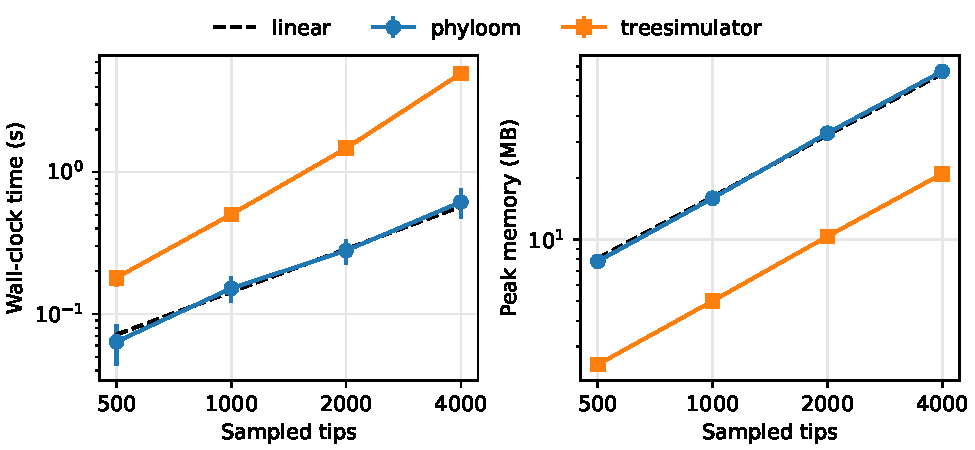
\includegraphics[width=0.8\linewidth]{figures/tree_size.pdf}
  \caption{Wall-clock time (left) and peak memory (right) to generate a tree
    with a given number of sampled tips under a constant-rate BD model
    ($R_0=3$, $\mu=0.4$, $p=0.5$), for \texttt{phyloom} and
    \texttt{treesimulator} (mean $\pm$ s.d.\ over 5 replicates; log--log
    axes). The dashed line has slope 1, i.e.\ linear scaling, fitted
    to the \texttt{phyloom} values. Benchmarks were run single-threaded
    on a MacBook with an Apple M3 chip and 16\,GB RAM, with Python 3.10.}
  \label{fig:benchmark}
\end{figure}

\bibliographystyle{unsrtnat}
\bibliography{../references}

\end{document}
